\documentclass[tikz,border=10pt]{standalone}
\begin{document}
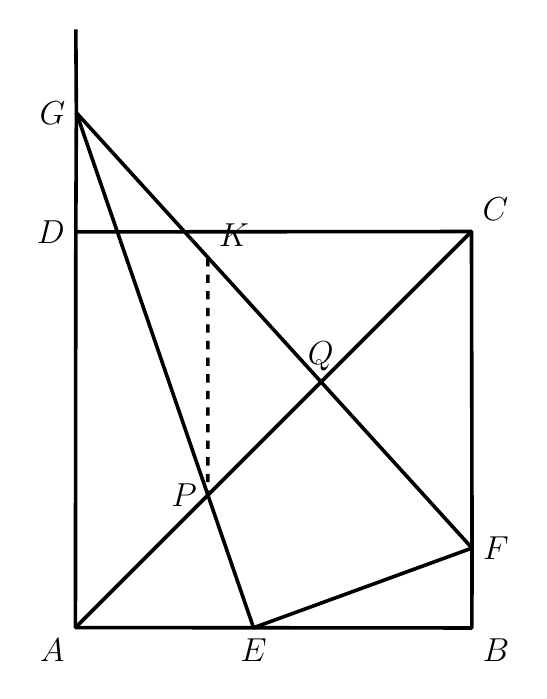
\begin{tikzpicture}[line width=1.3pt, line join=round,
  every node/.style={font=\fontsize{12.5}{15}\selectfont}]
\coordinate (A) at (-2.512,-3.468);
\coordinate (B) at (2.523,-3.473);
\coordinate (C) at (2.518,1.562);
\coordinate (D) at (-2.507,1.557);
\coordinate (F) at (2.525,-2.458);
\coordinate (G) at (-2.500,3.071);
\coordinate (K) at (-0.830,1.226);
\coordinate (P) at (-0.831,-1.786);
\coordinate (Q) at (0.603,-0.347);
\coordinate (GeoTailG) at (-2.507,4.128);




\coordinate (E) at (-0.250,-3.470);


\draw (A) -- (B) -- (F) -- (C) -- (D) -- cycle;


\draw (D) -- (G) -- (GeoTailG);


\draw (A) -- (C);


\draw (G) -- (F);
\draw (G) -- (E);
\draw (E) -- (F);


\draw[dashed] (K) -- (P);


\node[left] at (G) {$G$};
\node[left] at (D) {$D$};
\node[below left] at (A) {$A$};
\node[below] at (E) {$E$};
\node[below right] at (B) {$B$};
\node[above right] at (C) {$C$};
\node[right] at (F) {$F$};
\node[above right] at (K) {$K$};
\node[left] at (P) {$P$};
\node[above] at (Q) {$Q$};
\end{tikzpicture}
\end{document}
